\documentclass[12pt, letterpaper]{article}
\usepackage[utf8]{inputenc}
\usepackage[margin=1in]{geometry}
\usepackage[super]{nth}

\usepackage{lineno}
\usepackage[
singlelinecheck=false
]{caption}
\usepackage{amsmath}
\usepackage{amsfonts}
\usepackage{bm}
\usepackage{bbm}
\usepackage{graphicx}
\usepackage{csvsimple}
\usepackage[section]{placeins}
\usepackage{lineno}
\usepackage{natbib}
\usepackage[T1]{fontenc}
\usepackage[breaklinks]{hyperref}
\usepackage{microtype}

\title{Estimating F-statistics in a probabilistic PCA space}
\author{Divyaratan Popli, Benjamin M. Peter}
%\date{5 August 2021}
\linenumbers

\setlength{\parskip}{1em}
\setlength{\parindent}{0em}

\newcommand{\BZ}{\mathbf{Z}}
\newcommand{\BD}{\mathbf{D}}
\newcommand{\BN}{\mathbf{N}}
\newcommand{\BH}{\mathbf{H}}
\newcommand{\Btheta}{\pmb{\theta}}


\hbadness=99999
\begin{document}

\maketitle


\begin{abstract}

\noindent Principal component analysis (PCA) and F-statistics are routinely used in population genetic and archaeogenetic studies. However, these are closely related analyses and reveal the same biological signal. Here, we present a statistical framework to combine them into a joint analysis. In particular, we discuss the differences of probabilistic PCA and ordinary PCA, and show that F-statistics are more naturally interpreted in a probabilistic PCA framework. We also show that individual-based F-statistics can be accurately estimated from probabilistic PCA in the presence of large amounts of missing data. We present preliminary results using simulations and published data, and show that this joint estimation framework addresses  limitations of estimating F-statistics and PCA independently.

\end{abstract}

\section{Introduction}
A crucial first goal in any population genetic analysis of a natural population is to describe the observed genetic variation in the system. A major topic of population genetics is to link these patterns of variation with the underlying processes, including genetic drift, migration and selection.

Admixture, along with other events in the evolutionary history, shapes the genetic diversity of populations. An important goal of many population genetic studies is to identify the admixture events that have left their mark as patterns of variation in human populations. 

There are several methods available to make inferences about admixture events that explain the observed genetic diversity. These methods can be classified as local or global ancestry based. Local ancestry based methods infer ancestry at each locus and reveal recent history of each individual, but have low power to infer events in deep past \cite{vi_genome-wide_2023, brisbin_pcadmix_2012, price_sensitive_2009, sankararaman_estimating_2008}. Commonly used methods to infer global ancestry are Principal Component Analysis (PCA)  \cite{mcvean_genealogical_2009}, f-statistics \cite{patterson_ancient_2012, peter_admixture_2016}, MDS \cite{wang_comparison_2009}, and model based methods like STRUCTURE \cite{pritchard_inference_2000} and ADMIXTURE \cite{alexander_fast_2009}. 

PCA is a powerful method to visualize population structure but it can be difficult to interpret \citep{cavalli-sforza1993, novembre_stephens_2008, degiorgio_rosenberg2013}. In particular, the population structure in PCA is a function of expected pairwise coalescence times \citep{mcvean_genealogical_2009}, and thus is not explicitly tied to a particular scenario; different histories may yield similar or identical PCAs. 

Thus, parameter estimation, model comparisions and formal tests of admixture are usually not carried out in PCA. 

(add section here introducing the general idea of PCA, explain how it deals with error/noise  and difference between probabilistic and regular PCA. Possibly also explain how people use PCA as a QC-step to detect batch effects, and how that compares with PCA used for population structure (i.e. Ainash' question from your talk))

F-statistics are a useful tool to quantify population structure, and provide tests for admixture. Hence, a common pipeline in many population genetic studies is to analyze PCA plots to look for visible patterns that could be due to past admixtures, followed by formal test with F-statistics \cite{lazaridis_ancient_2014,lazaridis_genomic_2016}. F-statistics use population allele frequencies to test for admixture, and hence the accuracy of these tests is limited by the accuracy of allele frequency estimates \cite{peter_admixture_2016}. Whereas F-statistics estimates are robust when there are enough high quality samples, we show that low number of samples and missing data decrease the accuracy of these tests.

A major issue when working with ancient DNA is low number of individuals and missing data. This issue is exacerbated due to difficulty in assigning some of the individuals to discrete populations. Especially in the case of humans samples, we know that the genetic samples do not strictly belong to discrete populations, but form a continuous spectrum in the allele frequency space \cite{oteo-garcia_geometrical_2021}. Hence, it is a step in the right direction to think of a method to estimate F-statistics in a structure-aware framework. The easiest way to think about this is using PCA. PCA does not require assignment of individuals to discrete populations, and it has been shown that F-statistics can be estimated conveniently from distance between populations on PCA space \cite{peter_geometric_2022}. However, PCA distances are inaccurate when population sizes are small since PCA does not explicitly model sampling bias in the allele frequencies (see section XX). In addition, PCA is sensitive to missing data, and this makes it difficult to work with ancient DNA. 



In this study, we develop a statistical framework to estimate F-statistics between many populations in a probabilistic PCA framework.  that probabilistic PCA (PPCA) explicitly models the error due to the sampling bias in allele frequencies. In addition. we demonstrate that PPCA based framework is not sensitive to non-random missing data, and so it can be used to visualize individuals in PCA-space without having to project lower quality samples.

Finally, we show that PPCA provides a natural framework to estimate F-statistics with small sample-size and missing data. We show formal hypothesis tests for admixture and compare our results to admixtools2 cite{admixtools paper} on simulations. Finally we show the use of this framework on published datasets from neolithic Haak et al. and upper Paleolithic humans (Mateja). 

\section{Theory}

\subsection{F-statistics}
We follow the original notation \cite{patterson_ancient_2012}, and write the statistical estimates from empirical data as $f_2$, $f_3$ and $f_4$, and denote the theoretical values that depend only on the phylogenetic tree and the ascertainment scheme as $F_2$, $F_3$ and $F_4$. The three F-statistics are defined in the terms of population allele frequencies as follows:

\begin{align}\label{eq:f_intro}
F_2(X_1,X_2) &= \frac{1}{S}\sum_{l=1}^S(x_{1l} - x_{2l})^2\nonumber\\
F_3(X_1;X_2,X_3) &= \frac{1}{S}\sum_{l=1}^S(x_{1l} - x_{2l})(x_{1l} - x_{3l})\nonumber\\
F_3(X_1,X_2;X_3,X_4) &= \frac{1}{S}\sum_{l=1}^S(x_{1l} - x_{2l})(x_{3l} - x_{4l})\nonumber\\
\end{align}

\subsection{PCA}
\subsection{fstats and PCA: Ben's paper}

\subsection{Probabilstic PCA}
\subsection{PCA-Waaij}

We show that practically PCA and PPCA differ in the way that while PCA rotates the dataset, PPCA additionally models and removes noise from the data.

\begin{figure}[ht!]
    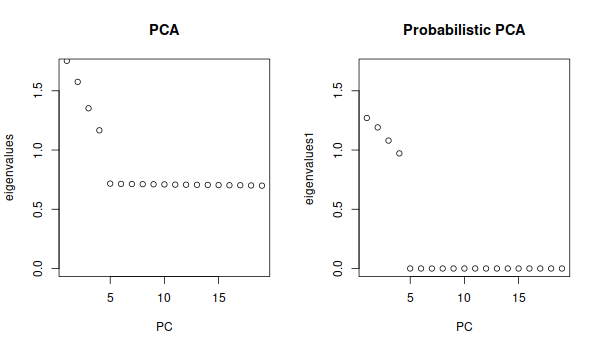
\includegraphics[width=16.5cm]{plots/pca_ppca.png}
    \centering
    \caption{Comparison of pca and ppca}
    \label{fig3:Comparison_READ_KIN}
\end{figure}

Next we show that PPCA/PCA-w is a natural framework to estimate f-statistics. Estimation of f2's compared for PCA, PPCA-1 PPCA2, admixtools.

\subsection{Probabilistic PCA and F-statistics}





\section{Results}


There are several tools available to understand genetic diversity, and can be classified as the tools that make minimal assumptions to summarize population structure, and the tools that infer demographic parameters. Former set of tools includes f-statistics \cite{patterson_ancient_2012}, PCA \cite{mcvean_genealogical_2009}, MDS \cite{wang_comparison_2009}, Structure \cite{pritchard}, Admixture  
- There are different tools to study diversity: 1) tools that make minimum assumptions like fstatistics, PCA, MDS, Structure, Admixture, 2) tools that can be used to infer demographic parameters.
- Many studies use PCA followed by f-statistics in their pipline. Peter et al., show that these analyses reveal the same biological signal, and can be done jointly.
- This framework has limitation: population allele frequencies are not known.
- Here we present an approach based on pPCA, and show that it is a more natural framework since it can take in account the errors associated with allele frequency estimation.

\subsection{Theory}
- f-statistics, and the sampling error terms in f2.
- PCA and relation to f-statstics.
- pPCA/PCA1 (Waaij et. al.) as a framework for dimentionality reduction taking in account the sampling error.

\subsection{results}
- Advantage in estimating PCs: Fig.1: PCA plot with standard errors

- Advantage in estimating f-statistics: We compare f-statistics from pPCA, PCA1, PCA, admixtools2 in terms of accuracy (and speed?). Fig.2: point estimates of f2's for slendr simulations where we have both ancient and modern populations. Fig.3: Examples of f4 test of treeness with different cases of migrations, we can also show a case of f3 test of admixture.

- Application to a published dataset (Fig.4)

\subsection{Discussion}
- One key advantage of this framework is that both point estimates and standard errors for PCA and fstatistics are estimated together in a consistent way.
- This is a step towards solving the issue with the assumption of discrete populations.
- This would be quite useful for cases where assigning individuals to populations can be difficult.
- Future work: 1) A faster way of estimating standard errors. 1) to get uncertainty from snp loading. 2) Hypothesis testing 

- This approach could also help with missingness as shown by Meisner et al. 
- pPCA makes it easy to analyse modern and ancient data together without having to project samples.

\subsection{Methods}
- Simulation method and parameters used


\section{Abstract}

Studies of genetic variation now routinely include data from thousands of individuals representing complex historical and temporal structure. Understanding and modeling patterns of genetic variation between large numbers of individuals and populations is thus a key challenge in the usage of genetic data to answer questions about evolutionary history. 
Principle Component Analysis (PCA) and F-statistics sensu Patterson are both widely used for this purpose, but are usually analyzed dis-jointly. Here, we present a new framework based on 
probabilistic PCA to jointly estimate principal component and F-statistics from large panels of data. A key advantage of our approach is that we can calculate individual-based F-statistics efficiently, and so population assignments become a result rather than an a priori assumption. Furthermore, probabilistic PCA provides a natural framework for incorporating missing data, a common issue in ancient DNA analyses. Taken together, our results greatly simplify the analysis of large population genetic data sets, and allow for fast data exploration and statistical testing in a unified and consistent framework.

\section{Background}

\subsection{Why study genetic diversity}
The genetic diversity of human populations has been shaped by historical and environmental factors over hundreds of thousands of years. Therefore, a key objective of population genetics is to analyze the observable variations and patterns in order to understand and reconstruct the demographic and evolutionary history of our species. 

\subsection{The general pipeline}

A general pipeline consists of a method to summarize the data with minimal assumptions. Examples are PCA, MDS, Structure, Admixture. These methods show a qualitative picture, but do not estimate a biologically meaningful parameter. And so, it is difficult to design statistical tests for the results of such methods. However, such qualitative results are generally followed by quantifiable methods based on f-statistics. F-statistics with 2,3, or 4 populations assumes a null-model as a tree-like structure and a deviation from the tree-like structure is represented the alternate model.

\subsection{PCA and fstatistics}
PCA is a method to rotate the dataset in a way that so that the axes that are analysed and plotted are aligned with the dimensions explaining the highest variation in the data. This is a way to do dimensionality reduction, and provides a way to do better data visualization. Ben[2020] showed that PCA and f-statistics are related, and   


\section{Introduction}
\subsection{Why combine pPCA and F-statistics?}

\paragraph{In case of no missing data}

- Calculating f-statistics between populations already assumes clustering of individuals into populations. PCA shows this clustering, but it would be useful to quantify the distance between individuals to filter for individuals that cluster, spot outliers, and identify substructures.

-Faster calculation of f-statistics, when only few PCs are used. Calculation of pPCA may take some time, but afterwards f-statistics is less time taking. And since people anyway do both PCA and f-statistics, overall this would reduce time.

-admixture proportions from f-statistics using pca. We can check if it's more reliable.
\paragraph{In case of missing data}

- In case of admixturegraphs, missing data may reduce total snps (although, missing sites would be less if allele frequencies are calculated from available individuals in populations). pPCA may help in cases with e.g., few ancient individuals from each population with a lot of missing data. 

- In case of ancient DNA, may help to include libraries with missing data instead of projecting them?
\newpage
\section{Practical application ideas}
This is a list of ideas we could pursue. Goal would be to pick a few that would be easiest to accomplish.
\begin{enumerate}
    \item Evaluate whether we use PPCA to calculate individual-based $F$-statistics accurately and fast?
    \begin{enumerate}
        \item in presence of missing data
        \item for multivariate analyses including qpadm/qpgraph
        \item include samples projected onto PCA
    \end{enumerate}
    \item Grouping individuals in populations
    
    \item Can we get confidence intervals on PCA?
        \begin{enumerate}
            \item Resampling SNPs
            \item Resampling individuals
            \item Calculate uncertainty based on SNP loadings
            \begin{enumerate}
                \item For SVD $\mathbf{X} = \mathbf{(UD)V}^T = \mathbf{PV}^T$, we might be able to use the correlation in the entries of $\mathbf{V}$ to estimate the ``effective'' number of SNPs
            \end{enumerate}
        \end{enumerate}
    \item Practical programming
        \begin{enumerate}
            \item Write software tool that jointly computes individidual-based F-stats and PCA
        \end{enumerate}
    \item Data analysis -- find a good data set or scenario to analyze
        \begin{enumerate}
            \item Standard Western Eurasian PCA
            \item Indian data
            \item Some application that Stephan / Wolfgang are working on
        \end{enumerate}
    \item Looking at qpadm/qpwave
        \begin{enumerate}
            \item qpadm projects samples into a subspace made from a subset of samples. As these samples are not orthogonal, this subspace is likely highly non-orthogonal and therefore tricky to work with. Doing PCA before doing qpadm could be helpful. 
        \end{enumerate}        
\end{enumerate}


\section{Projecting onto prob PCA}

For PCA, we can write $X_{[n \times p]} = USV^T$ and the PCs are given by $SV^T$. , and we would project by


\begin{align}
    X &= USV^T \\
    U^T X &= SV^T \\
    XVS^{-1} &= USV^TVS^{-1} \\
    &= U \\
    U^T Y &= Y_{proj}\\
    XVS^{-1}Y &= Y_{proj}
\end{align}
and we can project using $U^TY $ for new data $Y$. 


\newpage
\section{F-tests using Wishart-log-likelihoods}
Consider the $F_4$-statistic
\begin{align}
    F_4(A-B, C-D)&= Cov(A-B, C-D)\\ &= Cov(A, C) + Cov(B,D) - Cov(A,D) - Cov(B,D)\\
\end{align}


\subsection{PCA to Covariance matrix}
If we have a matrix of PCs, $\BP$, then $\mathbf{Y} = \BP\BP^T$ is an estimate of the covariance matrix. Consider the random variables $(A-B)$ and $(C-D)$. If we assume they are jointly normally distributed, then their joint distribution will again be normally distributed with mean zero and covariance matrix 
\begin{equation}
    \bf{X} = \begin{pmatrix} 
    y_{11} + y_{22} - 2 y_{12} & y_{13} + y_{24} - y_{14} - y_{23} \\
    y_{13} + y_{24} - y_{14} - y_{23} & y_{33} + y_{44} - 2 y_{34} &  \\
    \end{pmatrix}
\end{equation}
where the $y$ are the entries of the  covariance matrix obtained from the PCA. Practically, we can either first calculate $Y$ (if we want all $F$-stats), or first subset $\BP$ to the four pops involved.

The off-diagonal elements of $\MX$ are precisely the $F$-statistics we aim to calculate. And thus we set up a test to see whether they are zero.


\subsection{Derivation of the test statistic}
The sampling distribution of a covariance follows a Wishart distribution. This is a $p \times p$ - matrix-valued probability distribution that is parametrized by a degree-of-freedom parameter $n$ and a covariance matrix $\MS$, also of dimension $p \times p$. The simplest way to generate Wishart random variates is, 
\begin{equation}
    \MX = \sum_{i=1}^n Y_i Y_i^T
\end{equation}
where $Y_i \sim N(0, \MS)$. We also have 
\begin{align}
    E[\MX] &= n\MS \\
    mode(\MX) &= (n-p-1) \MS
\end{align}

The log-likelihood of a Wishart Distribution is

\begin{align}
    \log P(\MX | \MS, n) &= -\frac{np}{2} \log(2) -  \frac{n}{2}\log\left|\MS\right| - \Gamma_p\left(\frac {n}{2}\right ) + \frac{n-p-1}{2} \left|\MX\right| -\frac{1}{2}\operatorname{tr}({\MS}^{-1}\MX)\\
    &\propto  -\frac{n}2\log\left|\MS\right|   -\frac{1}{2}\operatorname{tr}({\MS}^{-1}\MX)\nonumber\\
    %&= -\frac{n}2 \log \left( \sigma_{11}\sigma_{22} - \sigma_{12}^2\right) - \frac{1}{2}\frac{\sigma_{22}x_{11} - 2\sigma_{12}x_{12} + \sigma_{11}x_{22}} {\sigma_{11}\sigma_{22} -  \sigma_{12}^2} 
    &= -\frac{n}2 \log \left( \sigma_{11}\sigma_{22} - \sigma_{12}^2\right) - \frac{1}{2}\frac{\sigma_{22}x_{11} + \sigma_{11}x_{22} -2 \sigma_{12}x_{12}} {\sigma_{11}\sigma_{22} -  \sigma_{12}^2} 
\end{align}
where the last step assumes a $2\times 2$ matrix. 
Under H0, we have $\sigma_{12} = 0$, therefore
\begin{align}
    \log P(\MX | \MS_0, n) &= -\frac{n}2 \log \left( \sigma_{11}\sigma_{22}\right) - \frac{1}{2}\left[\frac{x_{11}}{\sigma_{11}}  + \frac{x_{22}}{\sigma_{22}}\right] 
\end{align}
This likelihood is easily separatable and we can estimate $\sigma_{11}$ from $x_{11}$ and $\sigma_{22}$ from $x_{22}$ directly.

The log-likelihood-ratio statistic can then be calculated as 

\begin{align}
    R &= - 2 \log  \left( \frac{P(\MX | \MS_0, n)}{ P(\MX | \MS, n)} \right)  \nonumber\\
    &=2 [\log P(\MX | \MS, n) - \log P(\MX | \MS_0, n) ] \nonumber\\
    &=  n \log \left( \sigma_{11}\sigma_{22}\right) - n \log \left( \sigma_{11}\sigma_{22} - \sigma_{12}^2\right)  \nonumber\\
    &+  n\left[\frac{x_{11}}{\sigma_{11}}  + \frac{x_{22}}{\sigma_{22}}\right] 
    - n\frac{\sigma_{22}x_{11} + \sigma_{11}x_{22} -2 \sigma_{12}x_{12}} {\sigma_{11}\sigma_{22} -  \sigma_{12}^2} 
\end{align}
using the estimates $\sigma_{ij} = \frac{x_{ij}}{n}$ we get
\begin{align}
    R&\approx n \log \left( x_{11}x_{22}\right) - n \log \left( x_{11}x_{22} - x_{12}^2\right) + 2n - 2n  \nonumber\\
     &= n  \log \left( \frac{x_{11}x_{22}}{x_{11}x_{22} - x_{12}^2}  \right)
\end{align}
 A $\log(n^2)$ term in each of the log-terms cancels. The statistic $R$ is asymptotically $\chi^2$ distributed with one degree of freedom.

If we instead use the mode $\sigma_{ij} \approx \frac{x_{ij}}{n-3}$:

\begin{align}
    R&\approx n  \log \left( \frac{x_{11}x_{22}}{x_{11}x_{22} - x_{12}^2}  \right)
+2 (n-3) \frac{x_{11}x_{22} - x_{12}^2} {x_{11}x_{22} -  x_{12}^2} 
    - 2(n-3) \nonumber\\
     &= n  \log \left( \frac{x_{11}x_{22}}{x_{11}x_{22} - x_{12}^2}  \right)
\end{align}

\subsection{Comparison to Cavalli-Sforza \& Piazza, 1975}
The authors propose 
\begin{equation}
    R = \frac{|\MX|}{|\MS|}
\end{equation}
where $|\cdot|$ is the determinant. For $2 \times 2$ matrices,


\begin{align}
|\MX| &= x_{11}x_{22} - x_{12}^2 \\
|\MS| &= x_{11}x_{22} \\
    R &= \frac{ x_{11}x_{22} - x_{12}^2}{ x_{11}x_{22}} =1 - \frac{ x_{12}^2}{ x_{11}x_{22}}\\
    T &= -2 n \log (R) = 2 n \log \left( \frac{ x_{11}x_{22}}{ x_{11}x_{22} - x_{12}^2}\right)
\end{align}

The factor of 2 might be wrong..

\subsection{other statistics}
for $x_{12}$  small, we may further approximate
\begin{align}
         R &= n  \log \left( \frac{x_{11}x_{22}}{x_{11}x_{22} - x_{12}^2}  \right)\nonumber\\
            &= n  \log ( x_{11}x_{22}) - n\log ({x_{11}x_{22} - x_{12}^2} )\nonumber\\
            &= n  \log ( x_{11}x_{22}) - n\log \left[x_{11}x_{22} \left(1  - \frac{x_{12}^2}{x_{11}x_{22}} \right)\right]\nonumber\\
           &=n  \log \left( 1 - \frac{x_{12}^2}{x_{11}x_{22}}  \right) \nonumber\\
           &\approx  n \frac{x_{12}^2}{x_{11}x_{22}} 
\end{align}
This is the coefficient of determination, which is the square of the correlation coefficient
\begin{equation}
    r =  \sqrt{R/n} = \frac{x_{12}}{\sqrt{x_{11}x_{22}}}
\end{equation}

for which we have a $t$-distributed null
\begin{equation}
    r \sqrt{\frac{n-2}{1-r^2}} \sim t(n)
\end{equation}
The Fisher-Transform then yields
\begin{equation}
    \frac{1}{2} \log\left(\frac{1+r}{1-r}\right) = \arctan(r) \sim N(0,1)
\end{equation}
which simplifies to 
\begin{equation}
    \arctan(r) = \frac{1}{2} \log\left(\frac{\sqrt{x_{11}x_{22}} + x_{12}}{\sqrt{x_{11}x_{22}} - x_{12}}\right) 
\end{equation}
This statistic is normally distributed under the null-hypothesis.


in tests with a simple bivariate normal, all of them behaved equally well.


\newpage
\section{Calibrating the standard errors of $F$-stats}
Traditionally, the standard errors of F-stats are estimated using a block-Jackknife approach. However, the block size is usually hard to estimate, and may impact the resulting values.

\subsection{What do the standard errors measure?}
There are two types of uncertainty:
\begin{itemize}
    \item \textbf{sampling uncertainty}, that stems from the fact that we only have a small sample from each population. Because it depends on the sample, we expect these uncertainties to be independent for each sampled population
    \item \textbf{evolutionary uncertainty} there is also uncertainty due to the randomness in evolution. In particular, the realized mean allele frequencies in populations will be different from those expected under some model. 
\end{itemize}

\subsection{Covariance of $F_2$-statistics}
\begin{align}
    K &= Cov( (X_1- X_2)^2, (X_3 - X_4)^2 )  \nonumber\\
    &= Cov(X_1^2, X_3^2) + Cov(X_1^2, X_4^2) + Cov(X_2^2, X_3^2) + Cov(X_2^2, X_4^2) \nonumber\\
    &- 2\left [ Cov(X_1^2, X_3X_4) + Cov(X_2^2, X_3X_4) + Cov(X_3^2, X_1X_2) + Cov(X_4^2, X_1X_2)) \right]\nonumber\\
    &+ 4\left[ Cov(X_1X_2, X_3X_4)\right]\nonumber\\
\end{align}
At the same time, we have

\begin{align}
    F_4^2 &=  Cov(X_1 - X_2, X_3 - X_4) ^2 \nonumber\\
    &= \big[ Cov(X_1, X_3) + Cov(X_2, X_4) - Cov(X_1, X_4) - Cov(X_2, X_3)   \big]^2\nonumber\\
    &= Cov(X_1, X_3)^2 + Cov(X_2, X_4)^2 + Cov(X_1, X_4)^2 + Cov(X_2, X_3)^2  \nonumber\\
    &+2 \big[ Cov(X_1, X_3) Cov(X_2, X_4) + Cov(X_1, X_4) Cov(X_2, X_3)\big] \nonumber\\
    &-2 \big[ Cov(X_1, X_3) Cov(X_1, X_4) + Cov(X_1, X_3) Cov(X_2, X_3)\big] \nonumber\\
    &-2 \big[ Cov(X_2, X_4) Cov(X_1, X_4) + Cov(X_2, X_4) Cov(X_2, X_3)\big] \\
    &= (E[X_1^2] + E[X_2^2])(E[X_3^2] + E[X_4^2]) \nonumber\\
    &+2 \big[ E[X_1X_3]E[X_2X_4] + E[X_1 X_4] E[X_2 X_3]\big] \nonumber\\
    &-2 \big[ E[X_1 X_3] E[X_1 X_4] + E[X_1 X_3] E[X_2 X_3]\big] \nonumber\\
    &-2 \big[ EX_2 X_4] E[X_2 X_3] + E[X_2 X_4] E[X_2 X_3]\big] \\
    &= (E[X_1^2] + E[X_2^2])(E[X_3^2] + E[X_4^2]) \nonumber\\
    &+2 \big[ E[X_1X_3]  [ E[X_2X_4] - E[X_1 X_4]] +  E[X_2 X_3] [ E[X_1 X_4]  - E[X_1 X_3] ]\big] \nonumber\\
    &-2 \big[ EX_2 X_4] E[X_2 X_3] + E[X_2 X_4] E[X_2 X_3]\big] \nonumber\\
\end{align}
But we have $Cov(A,B) = E[ (A-E[A])(B-E[B])] = E[AB] - E[A]E[B]$ and 
\begin{align}
Cov(A, B)Cov(C, D) &= E[ (A-E[A]) (B-E[B])] E[(C-E[C])(D-E[D])]\nonumber\\
&= E[AB]E[CD] =  E[ABCD] - Cov(AB, CD)
\end{align}

\newpage
\section{Notes on PCA1 of van Waaij et al}
van Waaij et al. suggest at PCA on a matrix of the following form for PCA
\url{https://doi.org/10.48550/arXiv.2302.04596} (their PCA1). This approach is further motivated by eq 7 in \url{https://www.ncbi.nlm.nih.gov/pmc/articles/PMC6707457/}, which is a very technical (but probably useful) reference.

\begin{equation}
    \hat{\mathbf{H}} = \frac{1}{m}\mathbf{X}^T\mathbf{X} - \hat{\mathbf{D}},
\end{equation}
where $\MX$ is the (uncentered) genotype matrix and $\hat{\mathbf{D}}$ is a matrix of diagonal entries ``correcting'' heterozygosities and $m$ is the number of SNPs.

In particular $d_{ij} = 0 $ for $i \neq j$ and, 
\begin{equation}
    d_{ii} = d_i = \frac{1}{m}\sum_{k=1}^m x_{ik}(2-x_{ik}),
\end{equation}
for diploid data. The correction term given by Reich 2009 and Patterson 2012 is different by a factor of four:
\begin{equation*}
    d_{ii}' = \frac{1}{m}\sum_{k=1}^m \frac{x_{ik}(2-x_{ik})}{4} = \frac{d_{ii}}{4}
\end{equation*}.
The difference is explained that they use allele frequencies instead of genotypes, i.e. their approach would use (again for diploid data)
\begin{equation*}
    \hat{\mathbf{H}'} = \frac{1}{m}\frac{\mathbf{X}^T}{2}\frac{\mathbf{X}}{2} - \frac{\hat{\mathbf{D'}}}{4} = \frac{\hat{\mathbf{H}}}{4},
\end{equation*}
and so the parametrizations are equivalent, but will differ by a factor of four.

Thus, (TODO: double-check if rows/columns are aligned, sum should be over SNP)

\begin{subequations}\begin{align}
    h_{ii} &= \frac{1}{m}\sum_{k=1}^m x_{ik}^2 - d_i \\
    h_{ij} &= \frac{1}{m}\sum_{k=1}^m x_{ik}x_{jk} 
\end{align}\end{subequations}
Consider now
\begin{align}
    f_{ij} &= h_{ii} + h_{jj} - 2 h_{ij}\nonumber\\
     &= \frac{1}{m}\sum_{k=1}^m x_{ik}^2 - d_i + \frac{1}{m}\sum_{k=1}^m x_{jk}^2 - d_j - \frac{2}{m}\sum_{k=1}^m x_{ik}x_{jk}\nonumber \\
    &= \frac{1}{m} \sum_{k=1}^m (x_{ik} - x_{jk})^2 - d_i - d_j \\
    &= F_2(i,j)\nonumber
\end{align}

Hence the matrix $\hat{\mathbf{H}}$ can be used to estimate $F_2$-statistics (possibly instead of PPCA?).
The detailed justification of this can be found in \href{https://stats.stackexchange.com/questions/14002/whats-the-difference-between-principal-component-analysis-and-multidimensional}{this statsexchange post  that will need to be adapted}.

Thus, this might be a useful alternative to PPCA to calculate $F$-statistics:

\begin{enumerate}
    \item Calculate $\hat{\mathbf{H}} = \frac{1}{m}\mathbf{X}^T\mathbf{X} - \hat{\mathbf{D}}$
    \item Double-Center $\hat{\mathbf{H}}$: $\mathbf{H}_c = \mathbf{C}\hat{\mathbf{H}}\mathbf{C}$, where $\mathbf{C}$ is a centering matrix
    \item Obtain PCs using an eigendecomposition of $\mathbf{H}_c$: $\MP\MP^T = \mathbf{H}_c$
    \item Calculate $F_2$ from the smaller space $\MP$
\end{enumerate}

\section{Standard errors and effective number of SNPs}
An issue in calculating standard errors for $F$-statistics is that SNP are usually correlated, and so standard variance and standard error calculations will fail.

let us assume $n$ populations can be represented by some population structure model that is parameterized by some covariance matrix $\MX$. We do not observe SNPs, but rather we have a noisy sample $\MG_{[S \times n]}$ at $S$ loci.

Let, as above, denote the data matrix as $\MG$, which is a noisy version of an allele frequency matrix $\MX$, and we assume we can do a PCA on some estimate of $\hat{\MX}$ as 
$\ML\MZ = \hat{\MX}$ where $\ML$ are the orthonormal SNP-loadings and $\MZ$ are the PCs. For example, we could do that using probabilistic PCA or the Cabreros-Storey-PCA

We are interested in statistics of the form 
\begin{equation}
    F_{ij} = (X_i - X_j)^2
\end{equation}
which can be estimated from $\MG$ using the unbiased estimator of Patterson et al.
\begin{equation}
    f_{ij} = \frac{1}{S}\sum_{s=1}^n (g_{si} - g_{sj})^2 - H_i - H_j.
\end{equation}

alternatively, we can also obtain an estimate from the decomposition of  $\hat{\MX}$ as
\begin{equation}
    p_{ij} = \frac{1}{S}\sum_{p=1}^n (z_{si} - z_{sj})^2,
\end{equation}
this sum is over PCs. This estimator has thus the advantage that it can be computed a lot faster since typically $n \ll S$, and if $X$ is low-rank we can even truncate the sum

An issue is the calculation of the standard error of $f_{ij}$ and $p_{ij}$. A simple estimator is 
\begin{equation}
    \sigma_p = \sqrt{\frac{\operatorname{Var}(p_{ij})}{S} }
\end{equation}
a problem with $\sigma_p$ is that SNPs are not independent, and so the variance estimates are underestimated. For this purpose, a block-jackknife can be used.

We block data using a vector $b$, s.t $b_i = j$ means that the $i$-th SNP is in block $j$. For each block, we then have the pseudovalue 
$$\Tilde{f}^{(j)} = \frac{1}{m_j} \sum_s I[b_s =j] (x_{si} - x_{sj})^2  $$
where $I[\cdot]$ is an indicator and $m_j$ is the number of entries in block $j$.

then
\begin{equation}
    \sigma_f' = \sqrt{ \frac{1}{g} \sum_j \left[ \frac{m_j}{n-m_j}( \Tilde{f}^{(j)} - f)^2  \right] }
\end{equation}

This motivates the effective number of SNPs, 
\begin{equation}
    S_e = S \left(\frac{ \sigma_f}{\sigma_f'} \right)^2
\end{equation}

which gives the number of pseudo-independent observations.

\paragraph{simplifying block-JK}
Writing
$$f = \frac{1}{n}\sum_s (x_{si} - x_{sj})^2$$


\begin{align}
    \sigma_f'^2 &=  \frac{1}{g} \sum_j \left[ \frac{m_j}{n-m_j}( \Tilde{f}^{(j)} - f)^2  \right] \\
    &= \frac{1}{g} \sum_j \left[ \frac{m_j}{n-m_j} \left(  \left[ \frac{1}{m_j} \sum_s I[b_s =j] (x_{si} - x_{sj})^2\right] - f\right)^2  \right]\\
&= \frac{1}{g} \sum_j \left[ \frac{m_j}{n-m_j} \left(  \left[ \frac{1}{m_j} \sum_s I[b_s =j] (x_{si} - x_{sj})^2\right] - \left[\frac{1}{n}\sum_s (x_{si} - x_{sj})^2\right] \right)^2  \right]\\    
&= \frac{1}{g} \sum_j \left[ \frac{m_j}{n-m_j} \left(  \sum_s \left[ \frac{1}{m_j} I[b_s =j] (x_{si} - x_{sj})^2 - \frac{1}{n} (x_{si} - x_{sj})^2\right] \right)^2  \right]\\    
&= \frac{1}{g} \sum_j \left[ \frac{m_j}{n-m_j} \left(  \sum_s \left[ \frac{  I[b_s =j] n (x_{si} - x_{sj})^2 - m_j(x_{si} - x_{sj})^2 }{n m_j}   \right] \right)^2  \right]\\    
&= \frac{1}{g} \sum_j \left[ \frac{m_j}{n-m_j}\frac{1}{n^2m_j^2} \left(   \sum_s \left[  (x_{si} - x_{sj})^2 ( I[b_s =j] n  - m_j)    \right] \right)^2\right]\\    
&= \frac{1}{g} \sum_j \left[ \frac{m_j}{n-m_j}\frac{1}{n^2m_j^2} \left(   \sum_k (z_{ki} - x_{kj})^2 \underbrace{ \left\{n \sum_{s \in b}  l_{sk}^2  - m_j \right\}}_{ v_{bk}} \right)^2\right]\\    
\end{align}
Due to the indicator, this does not simplify easily.




This procedure can be run for any statistic. In particular, we could also do that on some estimates of $X_1$, i.e. columns of the denoised data:

\begin{align}
    \sigma^2_{x} &= \frac{1}{n} \sum_s (x_{s} -\bar{x})^2  \\
    &= \frac{1}{n} \sum_s \left( \sum_k  l_{sk} [z_{k1} - \bar{z}] \right)^2\\
    &= \frac{1}{n} \sum_s \left( \sum_k  l_{sk}^2 [z_{k1} - \bar{z}]^2 + 2\sum_k\sum_{k'}  l_{sk}l_{sk'} [z_{k1} - \bar{z}][z_{k'1} - \bar{z}] \right)^2\\  
    &= \frac{1}{n} \left [ \sum_k [z_{k1} - \bar{z}]^2 \left( \sum_s  l_{sk}^2\right)\right]  + \frac{2}{n} \left[ \sum_k\sum_{k'}  [z_{k1} - \bar{z}][z_{k'1} - \bar{z}] \left( \sum_s  l_{sk}l_{sk'}\right)\right ]  \\
    &= \frac{1}{n} \left [ \sum_k [z_{k1} - \bar{z}]^2 \right]
\end{align}

where we use the PCA-decomposition
\begin{equation}
    x_{s1} = \sum_k l_{sk} z_{k1}
\end{equation}
and the fact that the $l$ are orthonormal.

\section{Squared standard error/variance}
For  normal RV $X,Y$, $\COV{X^2}{Y^2} = 2 \COV{X}{Y}^2$.

Let $X_i^2$ be a vector of squared allele frequencies for individual $i$. We can think of $X_i$ as the location of the individual in an $s$-dimensional coordinate system, or, equivalently, the distance from an arbitrary point. This could either be the reference genome (represented by the zero vector), or the data centroid (for mean-centered SNPs). In either case, $ \sum_s x_{is}^2$ is the squared distance from that reference point, and $\sigma_i = \frac{1}{S} \sqrt{\sum_s x_{is}^2}$ is an estimate of the standard deviation per dimension. 


Alternative: Following the probabilistic PCA model, there are three sources of variation in the data:
\begin{enumerate}
    \item Biological variation due to shared ancestry. These are the principal components $\MP$ we aim to estimate
    \item Sampling error due to a finite number of loci. These are given by the $\ML$. Each entry of $\ML$ is normally distributed, but rows are typically not independent. Furthermore, for genetic data they are typically not independent.
    \item Sampling error due to finite samples from each population. These are given by the heterozygosities
\end{enumerate}

\begin{align}
x_{s} &= \sum_k \ML_k z_{sk} + \mu + \epsilon_s\\
x_{s} - x_{t} &= \sum_k \ML_k (z_{sk} - z_{lk}) +  \epsilon_s -  \epsilon_t\\
(x_{s} - x_{t})^2 &=  \left(\sum_k \ML_k (z_{sk} - z_{lk} ) +  \epsilon_s - \epsilon_t\right)^2\\
&= \sum_k(z_s - z_l)^2 + \epsilon_s^2 + \epsilon_t^2
\end{align}
because the error terms are independent of the $z_s$, and $\ML$ is an orthonormal basis such that $\sum_k {L_k}^2=1$ and $\sum_{k, k'} {L_k L_k'} = 0$

This shows that the \emph{sampling errors} are simply independent of the $F$-stats, and can be obtained e.g. from the heterozygosities (following Chen \& Storey, as in van Waaij et al). They also correspond to the ``correction terms''.

This is just o







\bibliographystyle{plain}
\bibliography{references.bib}





\end{document}


